\section{Related Work}
\label{sec:related_work}

If we assume that search targets are static in the search environment, the scan on a location decreases the estimated probability that there is some search target here.
Observations in a search process reduce the uncertainty of where search targets locate.
By measuring this type of uncertainty with information, a search agent can collect more information at non-observed locations than observed ones.
Information gathering is usually selected to measure the efficiency of a search task.
In this paper, we focus on path planning in a search task answers how to maximize information with limited time and resource by defining objective in forms of information evaluation \cite{goodrich2013toward}.

Research work on information maximization path planning focuses a lot on how to solve the optimization problems defined in large scale solution spaces in reasonable time.
\cite{levine2010information} imports ideas of RRT to an information-rich path planning problem, which targets at bringing good efficiency in online optimization in a continuous space.
Under a temporal logic constraint, \cite{JonesSchwagerBeltaICRA13scLTLInfo} use a receding horizon planning to solve an online information-gathering optimization problem.

\begin{figure}
\centering
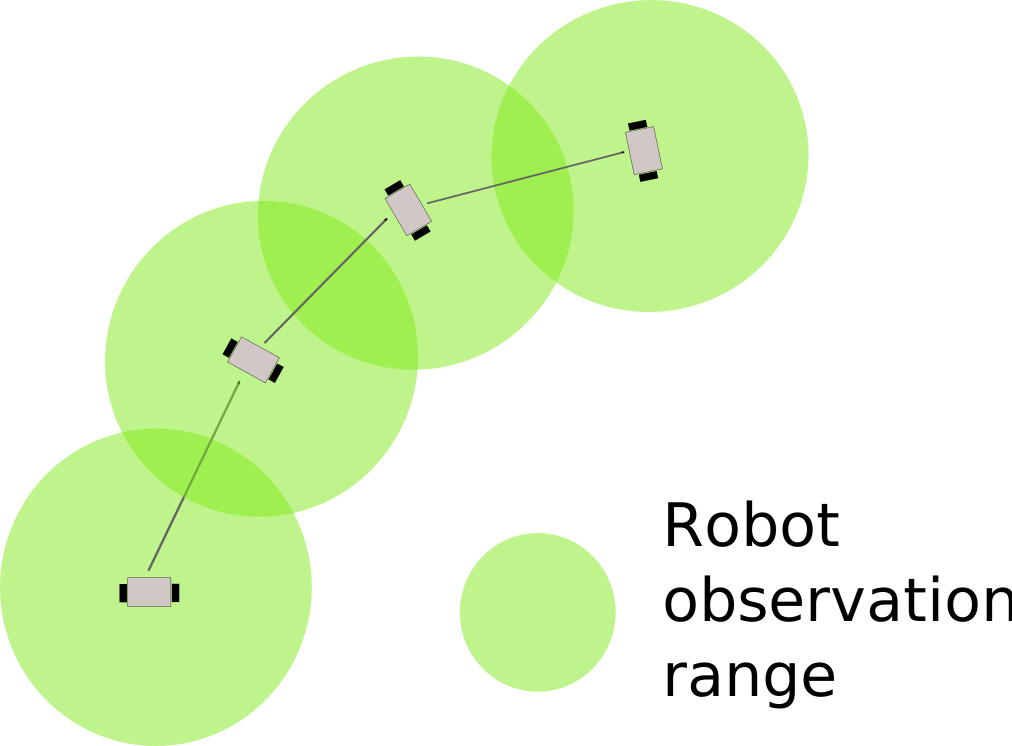
\includegraphics[width=0.4\linewidth]{./images/robotObservation.pdf}
\caption{Maximum coverage in robot observation.}
\label{fig:robotObservation}
\end{figure}

Usually the observation of a search agent covers a much larger region than the area occupied by the robot's body, which is shown in Figure \ref{fig:robotObservation}.
If we consider the observation as a covering range instead of a cell or a point, the overlaps between observation coverage at different time steps must be considered when measuring the total quantity of information.
Figure \ref{fig:robotObservation} gives an example.

Mutual information and conditional mutual information are commonly used to model the overlaps in measuring the total information \cite{singh2009efficient}.
This belongs to a \emph{maximum coverage problem}. 
Multiple sensors placement is one of the applications on information maximization.
In a sequential placement, the locations of placed sensors determine the increase on total information by adding a new sensor.
It is known to be a classical NP-hard combinatorial optimization problem \cite{megiddo1983maximum}.
The problem of maximum coverage on information measurement implies a property of ``nondecreasing submodularity''. 

Maximizing the score collected from a limited-length graph walk is usually known as an \emph{orienteering problem} \cite{Vansteenwegen20111}, in which the total score is a summation of the scores of visited vertices.
If the score function of a vertex has submodularity as in a \emph{maximum coverage problem}, the problem is defined as a \emph{submodular orienteering problem} \cite{chekuri2005recursive}.
A greedy approximation with known performance bound proposed in \cite{singh2009efficient} efficiently exploits the submodularity property of mutual information.
Similarly, in a branch and bound way, \cite{binney2012branch} apply greedy search to informative path planning.
Because the location of the robot at time $ t $ constrains the reachable location at time $ t+1 $, applying greedy algorithm with ``teleport'' assumption to the problem with this constraint can be extremely bad \cite{krause2012submodular}.
In non-teleport motion, \cite{chekuri2005recursive} import recursive greedy by converting to a knapsack constraint so that there is a time resource allocation on planning steps.

Due to the wingman constraint, the path planning of a robot wingman depends on a temporal-space synchronization requirement determined by the positions of a human through time.
The time allocation is fixed and depends on how the human's positions are sampled.
Thus we are not able to model time resource as budget in \cite{chekuri2005recursive}.   

We define the path planning of the robot wingman in a search task as an information maximization problem on a topological graph. We propose an algorithm to solve it as submodular orienteering . The algorithm is designed to produce acceptable robot performance and to be computed efficiently. We then use simulation to demonstrate the acceptable performance of the algorithm and computation efficiency. 
